\section{Performance characteristics of PET scanners}
\label{sec.ppet}

A major goal of PET studies is to obtain a good quality and detailed image of an object. Several parameters associated with the PET scanner are critical to good quality image formation, including energy resolution (ER) spatial resolution (SP), sensitivity, noise, scattered radiations, and contrast. These parameters are interdependent, and if one parameter is improved, one or more of the others may be compromised. We present a brief summary below.

\subsection{True, scattered and random coincidences in a PET detector}

\begin{figure}[!bthp]
	\centering
	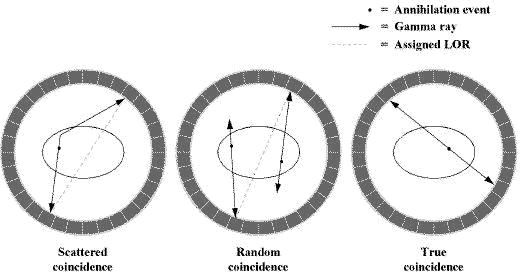
\includegraphics[scale=1.0]{img/MAPD_coincidencecategories.jpg}
	\caption{\label{fig.coi} Coincidence detection principle in a PET detector.}
\end{figure}


The reconstruction of the image in a PET system requires crossing many LOR which in turn define one emission point in the area under study. LOR are formed by detecting the coincidence of two photons. Three types of coincidences, illustrated in Figure \ref{fig.coi} are relevant:

\begin{itemize}
\item {\bf True coincidences} occur when both photons from an annihilation event are detected by detectors, neither photon undergoes any form of interaction prior to detection, and no other event is detected within the coincidence time-window.
\item {\bf A scattered coincidence} is one in which one of the detected photons (sometimes both) has undergone at least one Compton scattering event prior to detection. Since the direction of the photon changes due to the scattering process, the resulting coincidence event will be, most likely produce a wrong LOR. Scattered coincidences add a background to the true coincidence distribution which changes slowly with position, decreasing contrast and causing the isotope concentrations to be overestimated. They also add statistical noise to the signal. The number of scattered events detected depends on the volume and attenuation characteristics of the tissue being imaged. The best way to reject scattered coincidences is to build a PET system based on detectors with excellent energy resolution, since the scattered photons have also lost a fraction of their energy, and can therefore be rejected by imposing that the measured energy is inside a narrow window around 511 keV.
\item {\bf Random coincidences} occur when two photons, not arising from the same annihilation event, impinge the detectors within the coincidence time window of the system. As with scattered events, the number of random coincidences detected also depends on the volume and attenuation characteristics of the object being imaged, and on the geometry of the camera. The distribution of random coincidences is fairly uniform across the field of view and will cause isotope concentrations to be overestimated if not corrected for. Random coincidences also add statistical noise to the data. The best way to reject random coincidences is to build a PET system based on detectors with excellent time coincidence resolution (CRT), since in this case one can impose a very narrow coincidence window, therefore minimizing the number of random coincidences which is proportional to CRT. 
\end{itemize}


%\subsection{Spatial resolution of the PET system}
%
%\begin{figure}[!bthp]
%	\centering
%	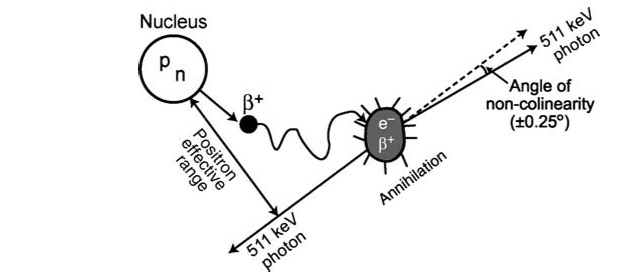
\includegraphics[scale=1.0]{img/range.png}
%	\caption{\label{fig.range} Positrons travel a distance before annihilation in the absorber and the distance increases with positron energy. Since positrons with different energies travel in zigzag directions, the effective range is the shortest distance between the nucleus and the direction of 511 keV photons. This effective range degrades the spatial resolution of the PET scanner.}
%\end{figure}
%
%The spatial resolution of a PET scanner is a measure of the ability of the device to faithfully reproduce the image of an object. It is empirically defined as the minimum distance between two points in an image that can be detected by the scanner. A number of factors contribute to the spatial resolution of the whole system.
%\begin{itemize}
%\item {\bf Individual detector resolution}: the scanner spatial resolution depends on the spatial resolution of the individual detectors used to build the system. Notice that for conventional solid scintillators one does not measure the longitudinal coordinate, $z$, (define along the line of flight of the photons), and therefore the resolution in $z$~depends of the longitudinal size (thickness) of the individual detectors.   
%\item {\bf Positron range}: the emitted positron travels a distance in tissue, losing most of its energy by interaction with atomic electrons and then is annihilated after capturing an electron. Thus, the site of emission differs from the site of annihilation as shown in Figure \ref{fig.range}. The distance (range) traveled by the positron increases with its energy, but decreases with the tissue density. Since the positrons are deflected after interaction with electrons resulting in a zigzag trajectory, the positron range is essentially an effective range, which is given by the shortest (perpendicular) distance from the emitting nucleus to the positron annihilation line. Furthermore, positrons are emitted with a distribution of energy, which also affects the effective range. The effective positron ranges in water for F-18 is 2.2 mm. Since coincidence detection is related to the location of annihilation and not to the location of the positron emission, an error  occurs in the localization of true position of the positron emission thus resulting in the degradation of spatial resolution. However, this contribution to the spatial resolution is small, of the oder of 0.2 mm for F-18.
%\item {\bf Noncolinearity}: another factor of concern is the noncolinearity that arises from the deviation of the two annihilation photons from the fact that the two 511 keV photons are not emitted at exactly 180$^\circ$ after the annihilation process because of some small residual momentum of the positron at the end of the positron range. The maximum deviation from the 180$^\circ$ direction is $\pm 0.25^\circ$. Thus, the observed LOR between the two detectors does not intersect the point of annihilation, but is somewhat displaced from it. This error  degrades the spatial resolution of the scanner and deteriorates with the distance between the two detectors that register the photons. The contribution from noncolinearity worsens with larger diameter of the ring, and it amounts to 1.8--2 mm for currently available 80--90 cm PET scanners.
%\end{itemize}

\subsection{Sensitivity}

The sensitivity of a PET scanner is defined as the number of counts per unit time detected by the device for each unit of activity present in a source. It is normally expressed in counts per second per microcurie (or megabecquerel) (cps/$\mu$Ci or cps/kBq). Assuming that dead time is small, sensitivity depends on the geometric efficiency and detection efficiency. The detection efficiency of a detector depends on the scintillation decay time, density, atomic number, and thickness of the detector material. Thus, for example, Lutetium Oxyorthosilicate (LSO) has a very large density (7.4 g/cc) which results in an attenuation length at 511 keV of 12 mm. LXe is less dense (3 g/cc), and has, therefore, a longer attenuation length, 36 mm at 511 keV. This implies that a LXe detector needs to be 3 times thicker than a LSO detector to achieve the same detection efficiency.

The geometric efficiency of a PET scanner is defined by the solid angle projected by the source of activity at the detector. The geometric factor depends on the distance between the source and the detector, the diameter of the ring and the number of detectors in the ring. Increasing the distance between the detector and the source reduces the solid angle and thus decreases the geometric efficiency of the scanner and vice versa. Increasing the diameter of the ring decreases the solid angle subtended by the source at the detector, thus reducing the geometric efficiency and in turn the sensitivity. Also the sensitivity increases with increasing number of rings in the scanner. This, in turn, requires a cost per detector as low as possible. LXe is 5 times cheaper than LSO (per unit detection, that is, taking into account that the detector must be 3 times thicker in the case of LXe than in the case of LSO) and can be more sparsely instrumented, at least for some applications, thus making it possible the construction of more rings, and therefore increasing the geometrical efficiency and the sensitivity. 

A simple formula for the sensitivity of a PET scanner is:
\begin{equation}
S = \frac{A \cdot \epsilon^2 \cdot e^{-\mu t} \cdot \xi}{4 \pi r^2} (cps/\mu Ci)
\label{eq.sensi}
\end{equation}
%
where $\xi = 3.7 \times 10^4$~is a numerical conversion factor, $A$~is the detector area seen by a point source to be image, $\epsilon$~is the detector efficiency (e.g, the fraction of the time the detector is alive, which in turn depends on the detector scintillating time and the response of sensors, multiplied by the fraction of events that are relevant for detection, e.g, photoelectric interactions), $\mu$~is the linear attenuation coefficient of 511 keV photons in the detector material, $t$~is the detector thickness. Notice that the factor $\epsilon^2$~comes from the need to form a coincidence with two detectors with efficiency $\epsilon$.

Equation \ref{eq.sensi} is valid for a point source at the center of a single ring scanner. For an extended source at the center of such scanners, it has been shown that the geometric efficiency is approximated as w/2r, where w is the axial width of the detector element and r is the radius of the ring. Thus the sensitivity of a scanner is highest at the center of the axial field-of-view (FOV) and gradually decreases toward the periphery. In typical PET scanners, there are also multiple rings and each detector is connected in coincidence with as many as half the number of detectors on the opposite side in the same ring as well as with detectors in other rings. Thus the sensitivity of multiring scanners will increase with the number of rings.


\subsection{Time of flight (TOF) application in a PET detector}

\begin{figure}[!bthp]
	\centering
	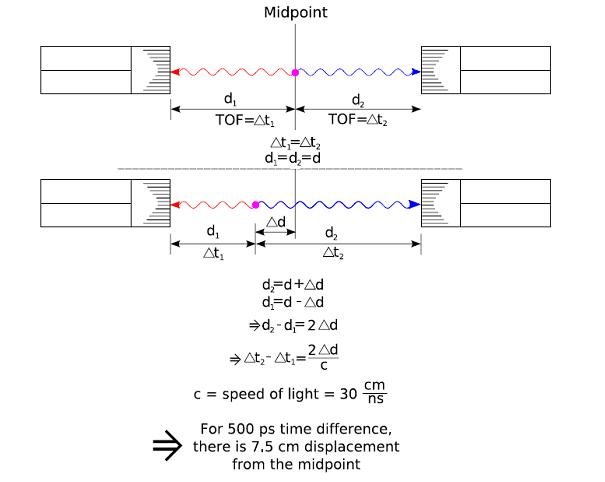
\includegraphics[scale=1.0]{img/MAPD_tofprinciple.jpg}
	\caption{\label{fig.tof} Time of flight (TOF) principle in a PET detector.}
\end{figure}

A Time-of-flight (TOF) PET scanner takes advantage of the difference in arrival times of two photons from the same annihilation event to infer spatial information of this event. 

To understand the principle of TOF applied to PET is important to recall that light travels 30 cm in 1 ns. Consider the situation illustrated in Figure \ref{fig.tof}. In principle one can measure the point of emission along the LOR by taking the time of flight difference between the arrival of the two photons. Since (Figure \ref{fig.tof}):
\begin{equation}
\Delta t = \Delta t_2 - \Delta t_1 = \frac{2 \Delta d}{c}
\end{equation}
%
and $c = 30 cm/ns$, it follows that the displacement from the mid point
$\Delta d$ is related with the TOF difference between the two photons $\Delta t$ and the speed of light $c$ as:

\begin{equation}
\Delta d =c \frac{2 \Delta t}{2}
\end{equation}

Thus, if one is able to measure $\Delta t$~ to a resolution of 500 ps (corresponding to the
best time resolution achieved by current commercial systems), the resulting precision in the
determination of $\Delta t$~is 7.5 cm, to be compared with the typical resolution achieved by
conventional PET, which is of the order of 5 mm. A $\Delta t$~resolution of 25 ps would yield a resolution of better than 4 mm, competitive with that achieved in conventional PET scanner, and therefore TOF could be used to determine directly the emission point. 

\begin{figure}[!bhtp]
	\centering
	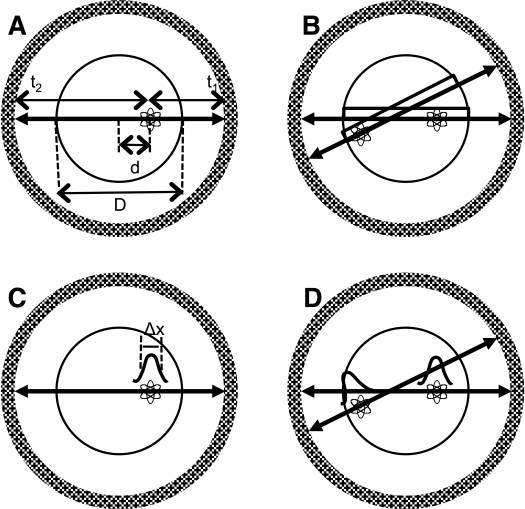
\includegraphics[scale=0.6]{img/tileshop.jpg}
	\caption{\label{fig.tile} (A) Emission point at a distance d from the center of the scanner within an object of diameter D. The two 511 keV photons are detected in coincidence at times t1 and t2. (B) Without precise TOF measurement a uniform probability along the LOR within the object is assumed for each emission point, leading to noise correlations over a portion of image space between the two events as shown in (B). (C) With TOF information the position of the emission point is localized along the LOR with a precision that is defined by a Gaussian distribution of width $\Delta x$. (D) Better localization of the two emission events along their individual LORs leads to reduced noise correlation of the events in image space image reconstruction. }
\end{figure}

In a TOF-PET scanner one uses good time-of-flight resolution to reduce the number of random coincidences, as illustrated in Figure \ref{fig.tile}. The principle is as follows. In a conventional PET without TOF one does not localize the emission point along the LOR. By collecting all possible LORs around the object (full angular coverage) and assuming uniform probability of the emission points lying along the full length of the LORs (and within object boundary), it is mathematically possible to reconstruct the emission object accurately (Figure \ref{fig.tile}, panels A and B). Knowledge of emission point locations along the LORs is not necessary to reconstruct the emission object. However, by assuming uniform probability of event location along the full LOR length, noise from different emission events gets forward and back projected during image reconstruction over many image voxels leading to increased noise correlation. Hence, the image signal-to-noise ratio (SNR) gets reduced.

In time-of-flight (TOF) PET the difference in the arrival times $(t_2 - t_1)$ of the two photons is measured with a precision $\Delta t$~(called coincidence timing resolution, CRT) that helps localize the emission point along the LOR within a small region of the object, as illustrated in  Figure \ref{fig.tile}, panel C. The uncertainty in this localization is determined by the CRT. The corresponding uncertainty in spatial localization $\Delta x$~ along the LOR is given by 
$\Delta x=c \times \Delta t/2$. As previously noted, if $\Delta x$~ is the same or smaller then the detector spatial resolution then in principle image reconstruction is not needed. Typically this spatial localization, however, is more than one order of magnitude worse than the detector spatial resolution, and hence image reconstruction is still necessary to produce tomographic images. However, during reconstruction, noise from different events is now forward and back projected over only a limited number of image voxels as defined by the spatial uncertainty, leading to reduced noise correlations and improved image signal-to-noise resolution (SNR) as illustrated in  Figure \ref{fig.tile}, panel D.


\begin{figure}[!bhtp]
	\centering
	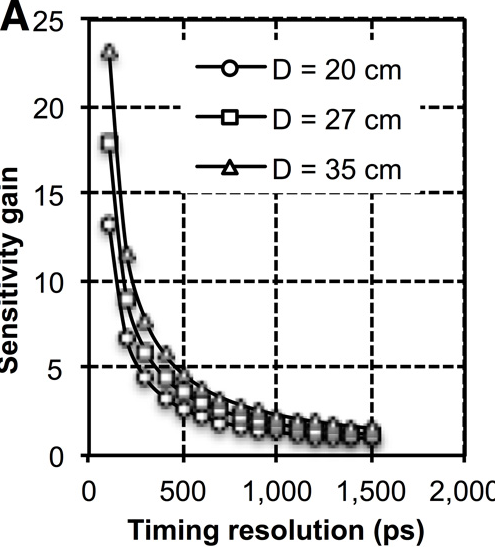
\includegraphics[scale=0.5]{img/SensiTof.png}
	\caption{\label{fig.sensi} Gain in sensitivity (defined in the text) as defined by $D/\Delta x$ plotted as a function of timing resolution for cylindrical ``phantoms'' with three different diameters.}
\end{figure}

With the knowledge that during the forward and back projection steps in image reconstruction noise will be spread over fewer voxels along the LOR (defined by $\Delta x$), it has been  shown  that the effective gain in sensitivity at the center of a uniform cylinder due to TOF information is given by $D/\Delta x$\footnote{ Snyder DL, Thomas LJ, Terpogossian MM. A mathematical model for positron emission tomography systems having time-of-flight measurements. IEEE Trans Nucl Sci. 1981;28:3575–3583.
12. Budinger TF. Time-of-flight positron emission tomography - status relative to conventional PET. J Nucl Med. 1983;24:73–76. [PubMed]}. Figure \ref{fig.sensi} shows a plot of this gain in sensitivity plotted as a function of timing resolution and for varying object sizes. As the object size increases or timing resolution improves the gain due to TOF PET increases. 

Consider as an example that one is performing a torso scan, ($D \sim 30$~cm). A PET capable of a CRT of 200 ps will result in $\Delta x = 3$~ cm and thus the gain in sensitivity may be as high as $30/3 = 10$). 
  
It follows that a PET scanner capable of a CRT in the range of 100 ps can improve the sensitivity by roughly a factor 10 w.r.t a conventional PET with no TOF measurement 


\subsection{Summary: main requirements for a PET scanner}

From the discussion above we can conclude that the 
main requirements for a PET scanner are: 

\begin{enumerate}
\item {\bf Dense detectors}, with high stopping power for 511 keV gammas.
\item {\bf Spatial resolution of sub mm to few mm}, depending on the application (small animal PET requires sub mm resolution while full body PET can be done with a resolution of few mm).
\item {\bf Energy resolution as good as possible}, to eliminate Compton coincidences.
\item {\bf High count rate capability ($\sim10^6$~ s$^{-1}$ per cm$^2$~ of detecting surface}, which results in minimizing scan times and/or doses.
\item {\bf Fast scintillating time}, which allows narrow CRT and possibilities TOF application. 
\item {\bf Large angular acceptance}, for torso, ``full body PET'', which in turn requires a large axial (along the patient's body) coverage. This requires cheap detection systems. 
\end{enumerate}